\documentclass[14pt]{extbook}
\usepackage{multicol, enumerate, enumitem, hyperref, color, soul, setspace, parskip, fancyhdr} %General Packages
\usepackage{amssymb, amsthm, amsmath, latexsym, units, mathtools} %Math Packages
\everymath{\displaystyle} %All math in Display Style
% Packages with additional options
\usepackage[headsep=0.5cm,headheight=12pt, left=1 in,right= 1 in,top= 1 in,bottom= 1 in]{geometry}
\usepackage[usenames,dvipsnames]{xcolor}
\usepackage{dashrule}  % Package to use the command below to create lines between items
\newcommand{\litem}[1]{\item#1\hspace*{-1cm}\rule{\textwidth}{0.4pt}}
\pagestyle{fancy}
\lhead{Module12L}
\chead{}
\rhead{Version A}
\lfoot{6131-5778}
\cfoot{}
\rfoot{test}
\begin{document}

\begin{enumerate}
\item{
Determine the horizontal and/or oblique asymptotes in the rational function below.\[ f(x) = \frac{3x^{2} -13 x + 12}{12x^{3} -25 x^{2} -18 x + 40} \]} \newpage
\item{
Determine the horizontal and/or oblique asymptotes in the rational function below.\[ f(x) = \frac{12x^{3} -13 x^{2} -19 x + 20}{-15x^{3} +52 x^{2} -48 x + 16} \]} \newpage
\item{
Determine the vertical asymptotes and holes in the rational function below.\[ f(x) = \frac{12x^{3} +55 x^{2} +18 x -40}{12x^{2} -5 x -25} \]} \newpage
\item{
Write an equation of a function that \textit{could} be represented by the graph below. Explain why your function could represent the graph.
\begin{center}
    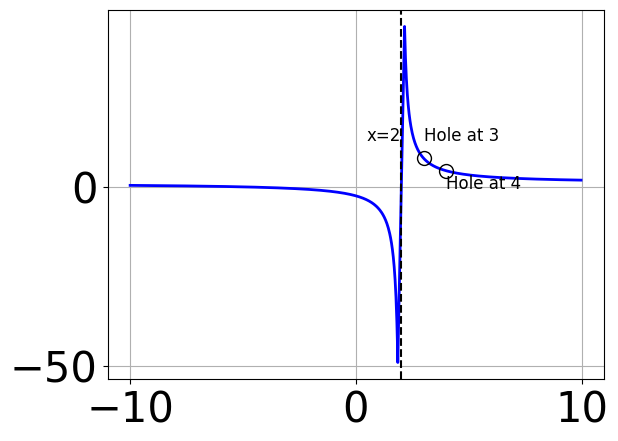
\includegraphics[width=0.5\textwidth]{../Figures/identifyGraphOfRationalFunctionA.png}
\end{center}
} \newpage
\item{
Write an equation of a function that \textit{could} be represented by the graph below. Explain why your function could represent the graph.
\begin{center}
    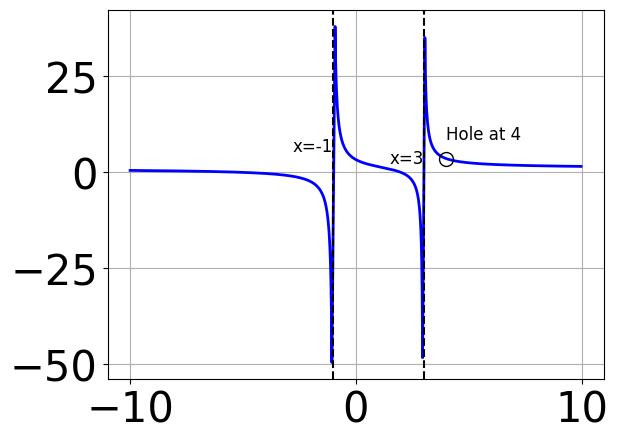
\includegraphics[width=0.5\textwidth]{../Figures/identifyGraphOfRationalFunctionCopyA.png}
\end{center}
} \newpage
\item{
Determine the horizontal and/or oblique asymptotes in the rational function below.\[ f(x) = \frac{6x^{3} +7 x^{2} -43 x -30}{2x^{2} +x -15} \]} \newpage
\item{
Determine the vertical asymptotes and holes in the rational function below.\[ f(x) = \frac{4x^{3} +12 x^{2} -7 x -30}{6x^{2} -x -12} \]} \newpage
\item{
Determine the vertical asymptotes and holes in the rational function below.\[ f(x) = \frac{6x^{3} -31 x^{2} +53 x -30}{12x^{2} -35 x + 25} \]} \newpage
\item{
Determine the vertical asymptotes and holes in the rational function below.\[ f(x) = \frac{8x^{3} +6 x^{2} -17 x -15}{6x^{2} -17 x + 12} \]} \newpage
\item{
Determine the horizontal and/or oblique asymptotes in the rational function below.\[ f(x) = \frac{6x^{3} + x^{2} -27 x + 20}{2x^{2} +11 x + 15} \]} \newpage
\end{enumerate}

\end{document}